\section{Discussion}
\subsection{The capacitor as a function of charge}

As shown in Figure \ref{fig:results:exp1}, the capacitor's voltage $V_C$ is linearly proportional with the charge on the capacitor. Therefore, this experimental data is the evidence of the correctness of the $Q = CV$ relation. 

When the charge becomes larger, the data deviates from the graph, while the error bars still fall under the linear function. When the rod touches the sphere, it is charged to $1000 (V)$, and when the rod touches the capacitor, the charge is redistributed from the rod to the capacitor, until the potential becomes equal on the rod and the capacitor. With each rod touch, the capacitor gains potential difference, and therefore, less and less charge is transferred on the capacitor with each rod-touch, which leads to smaller capacitor voltage gain. This is the reason data deviates as more charge is transferred on Figure \ref{fig:results:exp1}. 

\subsection{The distribution of charge on a surface} \label{dis:exp2}
In the middle of the capacitor, the capacitor looks like an infinite charged conductor plane. Therefore, the electric field is uniform and homogeneous in the middle of the capacitor. From the symmetry and the Gauss' law, the surface charge density should be constant throughout the capacitor plate.

However, the plane analogy breaks on the edges of the capacitor. The geometry of the edge of the capacitor plate is difficult to analyze and evidently more surface charge is pushed towards the edges. This creates curly field lines and bumps on the edges (see Appendix \ref{appendix:preps:q1}). This explains the raise of surface charge density in Figure \ref{fig:results:exp2}, and is called \textbf{the fringing effect}.

The best-fit curve (the sigmoid) in Figure \ref{fig:results:exp2} was estimated purely mathematically. Though there is no way to explicitly calculate the formula for the surface charge density of the capacitor), the classical graduate-level electromagnetism book \cite[p.89]{jackson} calculated the surface charge density for a conducting charged disk:

\begin{equation*}
    \sigma = \frac{q}{2\pi a} \frac{1}{\sqrt{a^2 - \rho^2}}
\end{equation*}

The graph of this function is shown in Figure \ref{fig:discussion:jackson}.

\begin{figure}[H]
    \centering
    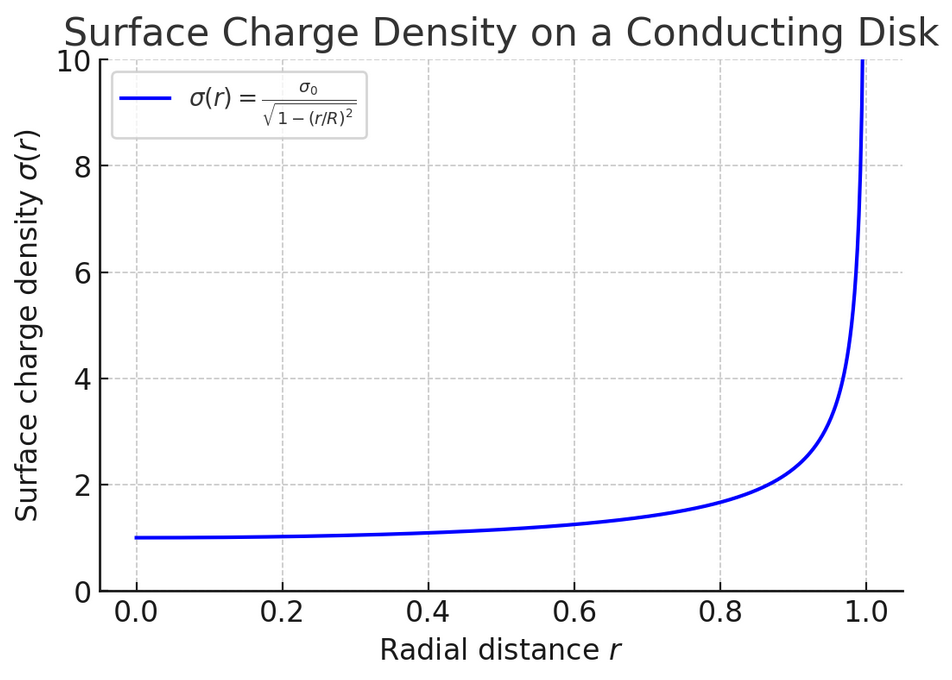
\includegraphics[width=0.8\linewidth]{capacitors/img/conducting_disk.png}
    \caption{Surface charge density of the conducting disk.}
    \label{fig:discussion:jackson}
\end{figure}

The graph in Figure \ref{fig:discussion:jackson} closely resembles the graph obtained experimentally in Figure \ref{fig:results:exp2}. This further solidifies the theory of electromagnetism. 
 

\subsection{The potential difference as function of the plate distance at constant charge}
By making graphs of the distance x versus the potential difference of the capacitor and $\frac{1}{x}$ versus $\frac{1}{V}$ we can understand the relation of these variables with regard to the capacitor and its capacitance.


For the graph of the potential difference as a function of the plate distance at constant charge we see a quadratic dependence. This can be explained by the fact that the capacitance of the capacitor is calculated by $C=\frac{\epsilon A}{x}$ (2) and that the energy stored in the capacitor charged to the potential is given by; $W=\frac{1}{2}CV^2$ (3). This fact together with the linear dependence of figure 4 creates a quadratic relation.

Looking at figure 7 we see that the relation of $\frac{1}{V}$ and $\frac{1}{x}$ is linear. This means we have a $\frac{1}{x}$ dependence. Which stands to reason as the capacitance is dependent on $\frac{1}{x}$ as seen in equation (2). 

 
If we now consider the fact that the electrometer itself also acts as a capacitor and that the capacitance of the electrometer can be seen as parallel to the capacitance plates of the capacitor, we can use the following equation;  \cite{manual}
\begin{equation} \label{eq:discussion:capacitance_addition}
    C_p= C_1+C_2 
\end{equation}
Where $C_p$ is the parallel capacitance.

Thus follows; $C_M=C_p-C_c$ where $C_M$ is the capacitance of the electrometer and $C_c$ is the capacitance of the capacitor.
$C_M=\frac{Q}{V}-\frac{\epsilon A}{x}$

For the capacitance of the capacitor itself we know; $C_c= \frac{\epsilon A}{x}$ This equation is only applicable at short distances, as shown in the figures above. 
 We know from Figure 4 in section 4.1 that the capacitor Voltage is linear with the amount of charges applied. This means $Q=\frac{\epsilon A}{x}=CV$.

The slope of the graph in figure 7 is $slope=\frac{x}{V}=a= 0.084 \pm 0.005$.  

We can now rewrite Q in the form of the slope so we get; 
$Q=\frac{\epsilon A}{slope V}$
From which follows; $\frac{Q}{V}=\frac{\epsilon A}{slope}$
This gives us; $C_M= \frac{\epsilon A}{slope}-\frac{\epsilon A}{x}$

Extrapolating the graph of figure 7 at small distances, we can estimate the magnitude of charge and the magnitude of capacitance $C_M$ of the electrometer.
Plugging in all the values, together with the value of $x=0.2 \pm 0.01$ gives us; 
$C_M= 1.9*10^-8 $

Since we know from error approximation that for $Z=aA+B$ with a = constant; $\Delta Z= a\Delta A +\Delta B$. And for the error in $1/x$ and $1/slope$ we will use the same error propagation as at section 4.3.

$C_M=(1.9 \pm 0.2)*10^-8 $
 


\subsection{Improvements}

The experiment was carried out in a laboratory that was not isolated from external interference. In fact, the laboratory members were not grounded and served as moving capacitors. Each time they moved or other not grounded and charged objects were turned on in the close vicinity to the lab equipment, it created external field $\mathbf{E}_{ext}$ that distorted the measurements of the very sensitive electrometer. This can be prevented by isolating the lab equipment and preferably putting it into the large Faraday cage, and grounding people inside the cage. 

Besides, the data was read of the electrometer using human eye which is prone to errors. It is better to directly read electrometer output by the computer and display the numbers.

In addition, the usage of more modern accurate equipment can significantly reduce the errors.
